\documentclass[a4paper,10pt,twoside]{article}
\usepackage[polish]{babel}
\usepackage[utf8]{inputenc}
\usepackage[T1]{fontenc}
\usepackage{indentfirst}
\usepackage[top=2.5cm, bottom=2.5cm, left=2.5cm, right=2.5cm]{geometry}
\usepackage{graphicx}
\usepackage{amsmath}
\usepackage{booktabs}

\begin{document}

\newcommand{\unit}[1]{\thinspace \mathrm{#1}}

\begin{center}
\bgroup
\def\arraystretch{1.5}
\begin{tabular}{|c|c|c|c|c|c|}
	\hline
	EAIiIB & \multicolumn{2}{|c|}{Piotr Morawiecki, Tymoteusz Paszun} & Rok II & {Grupa 3a} & {Zespół 6} \\
	\hline
	\multicolumn{3}{|c|}{\begin{tabular}{c}Temat: Mostek Wheatstone'a \end{tabular}} &
	\multicolumn{3}{|c|}{\begin{tabular}{c}Numer ćwiczenia: 35 \end{tabular}} \\
	\hline
	\begin{tabular}{@{}c@{}}Data wykonania:\\22.11.2017r.\end{tabular} & \begin{tabular}{@{}c@{}}Data oddania:\\29.11.2017r.\end{tabular} &
	\begin{tabular}{c}Zwrot do poprawki:\\\phantom{data} \end{tabular} & \begin{tabular}{c}Data oddania:\\\phantom{data}\end{tabular} &
	\begin{tabular}{@{}c@{}}Data zaliczenia:\\\phantom{data}\end{tabular} & \begin{tabular}{c}Ocena:\\\phantom{ocena}\end{tabular} \\[4ex]
	\hline
\end{tabular}
\egroup
\end{center}


\section{Cel ćwiczenia}

Celem ćwiczenia jest pomiar nieznanych oporów oraz kombinacji ich połączeń.

\section{Wstęp teoretyczny}

Wyznaczenie wartości napięć i prądów w poszczególnych częściach obwodu opiera się na trzech prawach:

\begin{itemize}
  \item I prawo Kirchoffa (prądowe prawo Kirchoffa) - w węzłach sieci, czyli w punktach połączeń trzech lub więcej przewodów, algebraiczna suma prądów wpływających równa jest zeru. 
  \item II prawo Kirchoffa (napięciowe prawo Kirchoffa) - suma różnic potencjałów w zamkniętej pętli obwodu (tzw. oczku) równa się zeru.
  \item Prawo Ohma - stosunek napięcia na końcach przewodu do wartości natężenia prądu jest wartością stałą, nazywaną opornością.
\end{itemize}

Aby znaleźć poszukiwane prądy powyższe warunki zapisujemy w formie układu odpowiedniej liczby niezależnych równań liniowych.

Analizując układ z rysunku \ref{fig:mostek} możemy wyprowadzić stosunek oporów:

$$ \frac{R_x}{R_2}=\frac{R_3}{R_4} $$

i przekształcając równanie:

$$ R_x = R_2\frac{R_3}{R_4} $$

gdzie $R_x$ jest poszukiwanym oporem.

\begin{figure}[!htp]
\centerline{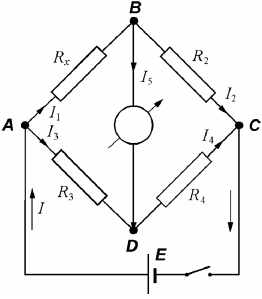
\includegraphics[scale=0.5]{mostek.png}}
\caption{Schemat oporowego mostka Wheatstone'a}
\label{fig:mostek}
\end{figure}

\section{Układ pomiarowy}

Na rysunku \ref{fig:uklad} przedstawiony jest przyrząd pomiarowy, w którym zastosowano drut oporowy wraz z linijką o dokładności $1 \unit{mm}$ służącą określeniu położenia punktu D od początku drutu (długość $a$). Długość drutu wynosi $l = 100 \unit{cm}$. Napięcie zasilania układu wynosiło $0,288 \unit{V}$. Opór $R_2$ stanowi opornica dekadowa. Symbolem $R_x$ oznaczono zestaw badanych oporników.

Jako, że w układzie zastosowano jednorodny drut oporowy równanie wartości poszukiwanego oporu możemy przedstawić jako:

$$ R_x = R_2\frac{a}{b} $$

Wiedząc, że $a + b = l$, możemy zapisać je w postaci:

$$ R_x = R_2\frac{a}{l - a} $$

\begin{figure}[!htp]
\centerline{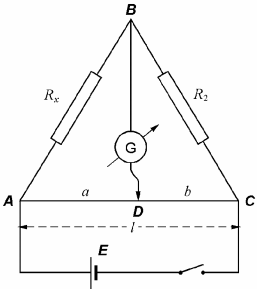
\includegraphics[scale=0.5]{uklad.png}}
\caption{Przyrząd pomiarowy - mostek Wheatstone'a z drutem oporowym}
\label{fig:uklad}
\end{figure}

\section{Wykonanie ćwiczenia}

\begin{enumerate}
  \item Podłączenie układu pomiarowego zgodnie ze schematem.
  \item Wykonanie dziesięciu pomiarów oporów dla różnych wartości $R_2$ dla każdego z badanych oporów.
\end{enumerate}

\newpage

\section{Wyniki pomiarów}


Niepewność pomiaru wartości oporu wyznaczamy przy pomocy wzoru:

$$ u(R_x) = \sqrt{\frac{\sum^n_{i=1}\left(R_i - \overline{R_x} \right)^2}{n(n-1)}} $$

	\begin{table}
		\centering
		\begin{tabular}{|l|r|r|r|r|r|r|r|r|r|r|}
			\hline
			$R_2[\Omega]$  & 10    & 11   & 12    & 13    & 14   & 9   & 8    & 7     & 6     & 5    \\
			\hline
			a[mm]  & 492   & 468  & 447 & 427   & 411  & 513  & 537  & 559   & 594   & 633   \\
			\hline
			$R_{x_1}$ & 9,69 & 9,68 & 9,70 & 9,69 & 9,77 & 9,48 & 9,28 & 8,87 & 8,78 & 8,62\\
			\hline                      
		\end{tabular}
		\caption{Pomiary dla opornika $R_{x_1}$}
		\label{tab:Rx1}
	\end{table}
$$\overline{R_{x_1}}=9,36 [\Omega]$$
$$u(R_{x_1})=0,37$$
\begin{table}
	\centering
	\begin{tabular}{|l|r|r|r|r|r|r|r|r|r|r|}
		\hline
		$R_2[\Omega]$  & 20    & 22   & 24    & 26    & 28   & 18   & 16    & 14     & 12     & 10   \\
		\hline
		a[mm]  & 490   & 466  & 450 & 430   & 413  & 502  & 532  & 553   & 604   & 644   \\
		\hline
		$R_{x_1}$ & 19,22 & 19,20 & 19,64 & 19,61 & 19,70 & 18,15 & 18,19 & 17,32 & 18,30 & 18,09\\
		\hline                      
	\end{tabular}
	\caption{Pomiary dla opornika $R_{x_2}$}
	\label{tab:Rx1}
\end{table}
$$\overline{R_{x_2}}=18,74 [\Omega]$$
$$u(R_{x_2})=0,73$$
\begin{table}
	\centering
	\begin{tabular}{|l|r|r|r|r|r|r|r|r|r|r|}
		\hline
		$R_2[\Omega]$  & 30    & 33   & 36    & 39    & 42   & 27   & 24    & 21     & 18     & 15   \\
		\hline
		a[mm]  & 516   & 502  & 484 & 474   & 449  & 532  & 571  & 609   & 666   & 700   \\
		\hline
		$R_{x_1}$ & 31,98 & 33,27 & 33,77 & 33,15 & 34,23 & 30,69 & 31,94 & 32,71 & 36,89 & 35,68\\
		\hline                      
	\end{tabular}
	\caption{Pomiary dla opornika $R_{x_3}$}
	\label{tab:Rx1}
\end{table}
$$\overline{R_{x_3}}=33,53 [\Omega]$$
$$u(R_{x_3})=1,41$$
\begin{table}
	\centering
	\begin{tabular}{|l|r|r|r|r|r|r|r|r|r|r|}
		\hline
		$R_2[\Omega]$  & 30    & 33   & 36    & 39    & 42   & 27   & 24    & 21     & 18     & 15   \\
		\hline
		a[mm]  & 492   & 470  & 449 & 430   & 412  & 508  & 547  & 576   & 620   & 658   \\
		\hline
		$R_{x_1}$ & 31,98 & 33,27 & 33,77 & 33,15 & 34,23 & 30,69 & 31,94 & 32,71 & 36,89 & 35,68\\
		\hline                      
	\end{tabular}
	\caption{Pomiary dla opornika $R_{x_1}$ i $R_{x_2}$ szeregowo}
	\label{tab:Rx1}
\end{table}
$$\overline{R_{x_{1,2szer}}}=29,01 [\Omega]$$
$$u(R_{x_{1,3szer}})=0,36$$
\begin{table}
	\centering
	\begin{tabular}{|l|r|r|r|r|r|r|r|r|r|r|}
		\hline
		$R_2[\Omega]$  & 6  & 7    & 8     & 9     & 10   & 5    & 4     & 3      & 2      & 1    \\
		\hline
		a[mm]  & 506   & 469  & 442 & 413   & 387  & 513  & 548  & 607   & 677   & 755   \\
		\hline
		$R_{x_1}$ & 6,14  & 6,18  & 6,34  & 6,33  & 6,31  & 5,27  & 4,85  & 4,64  & 4,19  & 3,08 \\
		\hline                      
	\end{tabular}
	\caption{Pomiary dla opornika  $R_{x_1}$ i $R_{x_2}$ rownolegle}
	\label{tab:Rx1}
\end{table}
$$\overline{R_{x_{1,2rown}}}=5,33 [\Omega]$$
$$u(R_{x_{1,2rown}})=0,93$$
	\begin{table}
		\centering
		\begin{tabular}{|l|r|r|r|r|r|r|r|r|r|r|}
			\hline
			$R_2[\Omega]$  & 40 & 45   & 50    & 55    & 60   & 35   & 30    & 25     & 20     & 15   \\
			\hline
			a[mm]  & 511   & 487  & 460& 437   & 415  & 540  & 585  & 599   & 667   & 722   \\
			\hline
			$R_{x_1}$ & 41,80& 42,72 & 42,59 & 42,69 & 42,56 & 41,09 & 42,29 & 37,34 & 40,06 & 38,96\\
			\hline                      
		\end{tabular}
		\caption{Pomiary dla opornika $R_{x_1}$ i $R_{x_2}$ růwnolegle i $R_{x_2}$ szeregowo}
		\label{tab:Rx1}
	\end{table}
$$\overline{R_{x_{12rown,3szer}}}=41,21 [\Omega]$$
$$u(R_{x_{12rown,3szer}})=1,48$$
\begin{table}
	\centering
	\begin{tabular}{|l|r|r|r|r|r|r|r|r|r|r|}
		\hline
		$R_2[\Omega]$  & 15& 17   & 19    & 21    & 23   & 13   & 11    & 9      & 7      & 5    \\
		\hline
		a[mm]  & 512   & 486  & 457 & 432 & 411  & 541  & 561  & 619 & 654   & 714   \\
		\hline
		$R_{x_1}$ & 15,74 & 16,07 & 16,00 & 15,97 & 16,05 & 15,32 & 14,06 & 14,62 & 13,23 & 12,48\\
		\hline                      
	\end{tabular}
	\caption{Pomiary dla opornika $R_{x_1}$ i $R_{x_2}$ i szeregowo i $R_{x_3}$ růwnolegle}
	\label{tab:Rx1}
	$$\overline{R_{x_{12oůwn,3szer}}}=14,95 [\Omega]$$
	$$u(R_{x_{12rown,3szer}})=1,08$$
\end{table}

\newpage

\section{Opracowanie wyników}

\subsection{Połączenie szeregowe}

Wartość oporu przy szeregowym połączeniu oporów $R_{x_1}$ oraz $R_{x_2}$ możemy obliczyć stosując wzór na opór zastępczy:

$$ R_{szer} = R_{x_1} + R_{x_2} = 28,10 \unit{\Omega} $$

Niepewność z prawa przenoszenia niepewności:

$$ u(R_{szer}) = \sqrt{\left( \frac{\delta R_{szer}}{\delta R_1}u(R_1) \right)^2 + \left( \frac{\delta R_{szer}}{\delta R_2}u(R_2) \right)^2 }= \sqrt{u(R_1)^2 + u(R_2)^2} = 0,82 \unit{\Omega}$$


\subsection{Połączenie równoległe}

Wartość oporu przy szeregowym połączeniu oporów $R_{x_1}$ oraz $R_{x_2}$ możemy obliczyć stosując wzór na opór zastępczy:

$$ R_{row} = \frac{R_{x_1} R_{x_2}}{R_{x_1} + R_{x_2}} = 6,24 \unit{\Omega} $$

Niepewność z prawa przenoszenia niepewności:

$$ u(R_{row}) = \sqrt{\left( \frac{\delta R_{row}}{\delta R_1}u(R_1) \right)^2 + \left( \frac{\delta R_{row}}{\delta R_2}u(R_2) \right)^2 }= \sqrt{\left( \frac{R_{x_1}}{R_{x_1} + R_{x_2}} \right)^4 u(R_{x_1})^2 + \left( \frac{R_{x_2}}{R_{x_1} + R_{x_2}} \right)^4 u(R_{x_2})^2} = 0,33 \unit{\Omega} $$

\subsection{Połączenie mieszane 1}

Wartość oporu przy równoległym połączeniu oporów $R_{x_1}$ i $R_{x_2}$ oraz szeregowym dołączeniu oporu $R_{x_3}$ możemy obliczyć stosując wzór:

$$ R_{p_1} = R_{szer} + R_{x_3} = 39,78 \unit{\Omega} $$

Niepewność możemy obliczyć używając wzoru dla niepewności połączenia szeregowego:

$$ u(R_{p_1}) = 1,45 \unit{\Omega} $$

\subsection{Połączenie mieszane 2}

Wartość oporu przy szeregowym połączeniu oporów $R_{x_1}$ i $R_{x_2}$ oraz równoległym dołączeniu oporu $R_{x_3}$ możemy obliczyć stosując wzór:

$$ R_{p_1} = \frac{R_{szer} R_{x_3}}{R_{szer} + R_{x_3}} = 15,29 \unit{\Omega} $$

Niepewność możemy obliczyć używając wzoru dla niepewności połączenia równoległego:

$$ u(R_{p_1}) = 0,45 \unit{\Omega} $$

\subsection{Analiza błędów}

Podczas analizy wyników nie znaleźliśmy błędów grubych. Natomiast analizując wykresy (rysunek ) możemy zauważyć, że zależność odległości $a$ od oporu wzorcowego w powtarzalny sposób odbiega od spodziewanej prostej. Wnioskujemy, że może być to związane z niejednorodnością zastosowanego drutu oporowego, bądź korozją wpływającą na opór punktu styku drutu z suwakiem.

\begin{figure}[!htp]
\centerline{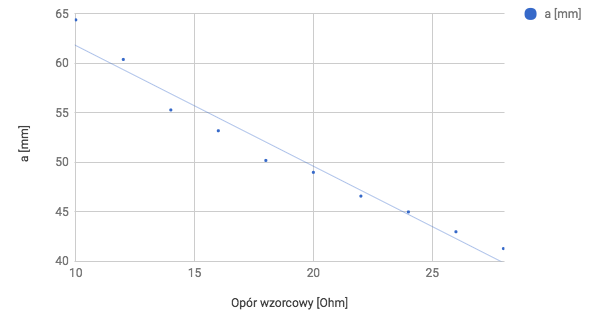
\includegraphics[scale=0.5]{wykres_r2.png}}
\caption{Zależność długości $a$ od oporu wzorcowego $R_2$}
\label{fig:wykres_r2}
\end{figure}

\begin{figure}[!htp]
\centerline{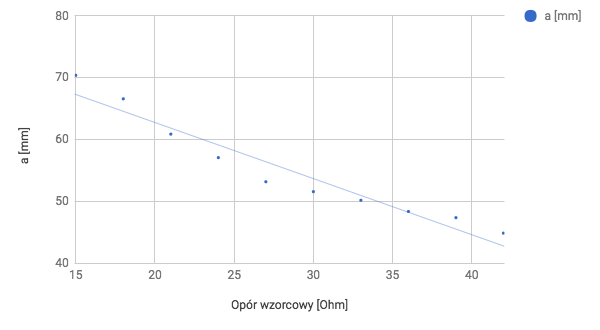
\includegraphics[scale=0.5]{wykres_r3.png}}
\caption{Zależność długości $a$ od oporu wzorcowego $R_3$}
\label{fig:wykres_r3}
\end{figure}

\begin{figure}[!htp]
\centerline{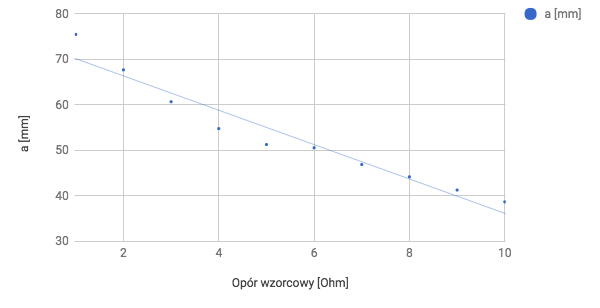
\includegraphics[scale=0.5]{wykres_r1_r2_par.png}}
\caption{Zależność długości $a$ od oporu wzorcowego $R_1, R_2$ połączonych równolegle}
\label{fig:wykres_r1_r2_par}
\end{figure}

\subsection{Ocena zgodności uzyskanych wyników}

\section{Wnioski}

\end{document}
